
\documentclass[12pt,a4paper]{article}
\usepackage{calc}% http://ctan.org/pkg/calc
\usepackage[
  letterpaper,%
  textheight={47\baselineskip+\topskip},%
  textwidth={\paperwidth-126pt},%
  footskip=75pt,%
  marginparwidth=0pt,%
  top={\topskip+0.75in}]{geometry}% http://ctan.org/pkg/geometry
\usepackage{fancyhdr}% http://ctan.org/pkg/fancyhdr

\usepackage{graphicx}
\usepackage[center]{subfigure}

\usepackage{hyperref}

\newcommand{\kpar}{k_{||}}
\newcommand{\kperp}{k_\perp}
\newcommand{\bvec}{\mathbf{b}}

\pagestyle{fancy}
%\fancyhead{}
\fancyfoot{}% Clear header & footer
%\fancyhead[L]{Electrostatic Ohm's law}% Set centered header
%\fancyhead[R]{ 22$^{nd}$ March 2014 }
\fancyfoot[C]{\thepage}% Set centered footer
\renewcommand{\headrulewidth}{0.5pt}% Add header rule

% Titling
\title{ 1D divertor model for detachment studies }% Your title
\author{ Ben Dudson }% Your author
\date{ 7$^{th}$ November 2015 }% Your date
\makeatletter
% Definition of proc.cls' \maketitle:
\def\@maketitle{% 
  \vbox to 1.25in{%
    \vskip 0.5em
    {\large \begin{tabular}[t]{ll}
        Title: & \@title \\
        Author: & \@author \\
        Date: & \@date \\
        Project: &
      \end{tabular}\par}
    \vfil}\noindent\hrulefill
    \vskip 2em}
\makeatother
\begin{document}
\maketitle % Produce title
\thispagestyle{fancy}% Override titling page style with fancy

This is a model of a 1D fluid, assuming equal ion and electron temperatures, no electric fields or currents. 

\section{Getting started}

First get a copy of development branch of BOUT++. You can download a tarball from \url{https://github.com/boutproject/BOUT-dev}, but it is strongly recommended you use Git:

\begin{verbatim}
$ git clone https://github.com/boutproject/BOUT-dev.git
\end{verbatim}

Configure and make BOUT-dev

\begin{verbatim}
$ cd BOUT-dev
$ ./configure
$ make
\end{verbatim}

The user manual for BOUT++ is in subdirectory of BOUT-dev called "manual", and contains more detailed
instructions on configuring and compiling BOUT++.
This will build the core library code, which is then used in each model or test case (see the examples/ subdirectory)

Put the sol1d tarball in the BOUT-dev/examples subdirectory. This isn't strictly necessary, but it makes the "make" command simpler (otherwise you add an argument \texttt{BOUT\_TOP=/path/to/BOUT-dev/} to make)

\begin{verbatim}
BOUT-dev/examples/ $ tar -xzvf bout-sol1d.tar.gz
BOUT-dev/examples/ $ cd bout-sol1d
BOUT-dev/examples/ $ make
\end{verbatim}

Hopefully you should see something like:

\begin{verbatim}
  Compiling  sol1d.cxx
  Compiling  div_ops.cxx
  Compiling  loadmetric.cxx
  Compiling  radiation.cxx
  Linking sol1d
\end{verbatim}

Here the main code is in "sol1d.cxx" which defines a class with two methods: \texttt{init()}, which is run once at the start of the simulation to initialise everything, and \texttt{rhs()} which is called every timestep. The function of rhs() is to calculate the time derivative of each evolving variable: In the \texttt{init()} function the evolving variables are added to the time integration solver (around line 100). This time integration sets the variables to a value, and then runs \texttt{rhs()}. On line 415 of
\texttt{sol1d.cxx} you'll see the density equation, calculating \texttt{ddt(Ne)}. \texttt{Ne} is the evolving variable, and \texttt{ddt()} is a function which returns a reference to a variable which holds the time-derivative of the given field. 

BOUT++ contains many differential operators (see \texttt{BOUT-dev/include/difops.hxx}), but work has been done on improving the flux conserving Finite Volume implementations, and they're not yet in the public repository. The functions \texttt{Div\_par\_FV} and \texttt{Div\_Par\_Diffusion} are defined in \texttt{div\_ops.hxx} and \texttt{div\_ops.cxx}.

The atomic rates are used in \texttt{sol1d.cxx} starting around line 345, and are defined in \texttt{radiation.cxx} and \texttt{radiation.hxx}. These were adapted from code Eva sent me a while ago.


To run a simulation, enter:
\begin{verbatim}
$ ./sol1d -d fluid
\end{verbatim}
This will use the "fluid" subdirectory for input and output. All the options for the simulation are in \texttt{fluid/BOUT.inp}. I've tried to comment it, but ask if anything's not clear.

The output should be a whole bunch of diagnostics, printing all options used (which also goes into log file BOUT.log.0), followed by the timing for each output timestep:

\begin{verbatim}
Sim Time  |  RHS evals  | Wall Time |  Calc    Inv   Comm    I/O   SOLVER

0.000e+00          2       1.97e-02    11.6    0.0    1.0   67.9   19.4
1.000e+03        967       8.98e-01    77.9    0.0    1.3    0.9   19.9
2.000e+03        287       2.02e-01    75.3    0.0    1.3    4.2   19.2
3.000e+03        213       1.52e-01    70.6    0.0    1.3    6.6   21.4
4.000e+03        211       1.46e-01    70.6    0.0    1.4    8.0   20.1
5.000e+03        333       3.25e-01    82.4    0.0    1.2    3.7   12.7
\end{verbatim}

The simulation time (first column) is normalised to the ion cyclotron frequency (this being part of a turbulence model),
which is stored in the output as  "\texttt{Omega\_ci}". So each output step is 1000. / \texttt{Omega\_ci} = 20.9 microseconds.
The number of internal timesteps is determined by the solver, and determines the number of times the \texttt{rhs()}
function was called, which is given in the second column. If this number starts increasing, it's often a sign of numerical problems.

To analyse the simulation, the data is stored in the "fluid" subdirectory along with the input. You can use IDL or Python to look at the "Ne", "NVi", "P" variables etc. which have the same names as in the \texttt{sol1d.cxx} code. See section~\ref{sec:output} for
details of the output variables and their normalisation. The evolving variables should each be 4D, but all dimensions are of size 1 except for the time and parallel index (200). Please see the BOUT++ user manual for details of setting up the Python and IDL reading ("collect") routines. 


\subsection{Examples}

{\bf diffusion}: A low powered (20 MW/m$^2$) test case, 100m long. Simple diffusive neutral model.

\noindent {\bf fluid}: Same as diffusive, but using a fluid neutral model.

In both cases the particle and power sources are uniform in the first half of the domain, and the cross-section has constant area.
The particle and power flux at the end of the source (nominally the X-point) can be set by changing these parameters:
\begin{verbatim}
[Ne] # Electron density 
flux = 9e22  # Particles per m^2 per second input
...
[P]    # Plasma pressure P = 2 * Ne * T
powerflux = 2e7  # Input power flux in W/m^2
\end{verbatim}

\section{Plasma model}

Equations for the plasma density $n$, pressure $p$ and momentum $m_inV_{||i}$ are evolved:

\begin{eqnarray*}
  \frac{\partial n}{\partial t} &=& - \nabla\cdot\left( \bvec V_{||} n\right) + S_n - S\\
  \frac{\partial}{\partial t}\left(\frac{3}{2}p\right) &=& -\nabla\cdot\mathbf{q} + V_{||}\partial_{||}p + S_p - E - R \\
  \frac{\partial}{\partial t}\left(m_i nV_{||}\right) &=& -\nabla\cdot\left(m_inV_{||}\bvec V_{||}\right) - \partial_{||} p - F\\
  j_{||} &=& 0 \\
  T_i &=& T_e = \frac{1}{2}\frac{p}{en} \\
  \mathbf{q} &=& \frac{5}{2}p\bvec V_{||} - \kappa_{||e}\partial_{||}T_e
\end{eqnarray*}

Which has a conserved energy:
\[
\int_V \left[ \frac{1}{2}m_inV_{||i}^2 + \frac{3}{2}p \right] dV
\]

\section{Non-uniform mesh}

An example of using a non-uniform grid is in \texttt{diffusion\_pn}.
The location $l$ along the field line as a function of normalised cell index $y$,
which goes from $0$ at the upstream boundary to $2\pi$ at the target, is
\begin{equation}
  l = L\left[ \left(2 - \delta y_{min}\right)\frac{y}{2\pi} -\left(1-\delta y_{min}\right)\left(\frac{y}{2\pi}\right)^2\right]
\label{eq:nonuniform_l}
\end{equation}
where $0<\delta y_{min}<1$ is a parameter which sets the size of the smallest grid cell, as a fraction
of the average grid cell size. The grid cell spacing $\delta y$ therefore varies as 
\begin{equation}
\delta y = \frac{L}{N_y} \left[ 1 + \left(1-\delta y_{min}\right)\left(1-\frac{y}{\pi}\right)\right]
\end{equation}
This is set in the BOUT.inp settings file, under the \texttt{mesh} section:
\begin{verbatim}
dy = (length / ny) * (1 + (1-dymin)*(1-y/pi))
\end{verbatim}
In order to specify the size of the source region, the normalised cell index $y$ at which
the location $l$ is a given fraction of the domain length must be calculated. This is done by
solving for $y$ in equation~\ref{eq:nonuniform_l}.
\begin{equation}
y_{xpt} = \pi\left[2 - \delta y_{min} - \sqrt{\left(2-\delta y_{min}\right)^2 - 4\left(1-\delta y_{min}\right) f_{source}}\right]/\left(1-\delta y_{min}\right)
\end{equation}
which is calculated in the BOUT.inp file as
\begin{verbatim}
y_xpt = pi * ( 2 - dymin - sqrt( (2-dymin)^2 - 4*(1-dymin)*source ) ) / (1 - dymin)
\end{verbatim}
where \texttt{source} is the fraction $f_{source}$ of the length over which the source is spread.
This is then used to calculate sources, given a total flux. For density:
\begin{verbatim}
source = (flux/(mesh:source*mesh:length))*h(mesh:y_xpt - y)
\end{verbatim}
which switches on the source for $y < y_{xpt}$ using a Heaviside function, then divides the flux
by the length of the source region $f_{source}L$ to get the volumetric sources.

\section{Boundary conditions}

At the midplane (upstream) boundary, no-flow boundaries are implemented:
\begin{eqnarray}
  \partial_{||}n &=& 0 \\
  \partial_{||}p &=& 0 \nonumber \\
  V_{||} &=& 0 \nonumber \\
  \partial_{||}n_n &=& 0 \nonumber
\end{eqnarray}
and hence $\partial_{||}T = 0$ and $\mathbf{q} = 0$.

At the target plate, normal sheath boundary conditions are applied, so velocity at the sheath entrance
is sonic:
\begin{equation}
V_{||}^{sheath} \ge C_s
\end{equation}
If the velocity just in front of the sheath is supersonic, then a zero-gradient boundary condition is used, but if
the flow in front of the sheath is subsonic then the sound speed is used. The flux of ions to the wall is therefore 
\begin{equation}
\Gamma = n^{sheath}V_{||}^{sheath}
\end{equation}

The flux of particles is assumed constant (i.e. sources/sinks neglected)
  \begin{eqnarray*}
   \partial_{||} \left( nV_{||} \right) &=& 0 \rightarrow n_{sheath} = V_{||,0} n_0 /  V_{||,sheath} \\
   \partial_{||} T &=& 0
 \end{eqnarray*}
 [Note: Important to limit $n_{sheath} \ge 0$ for case when $V_{||,0} < 0$]
 This will result in a heat flux from the fluid equations of
  \begin{eqnarray*}
  q_{fluid} &=& \left[\frac{5}{2}e\left(T_e + T_i\right) + \frac{1}{2}m_i V_{||,sheath}^2\right]n_{sheath}V_{||,sheath} \\
  &=& 6eTn_{sheath}V_{||,sheath} \rightarrow \gamma = 6
  \end{eqnarray*}
  which over-estimates the ion cooling, andunder-estimates electron cooling.
  Therefore, additional heat flux is removed from the pressure in the final cell
  \[
  q_{cooling} = \left(\gamma - 6\right)eTn_{sheath}V_{||,sheath}  \qquad \left( \gamma \ge 6 \right)
  \]
  
\subsection{Old boundary conditions}

An older version of the code is retained as \texttt{sol1d-bc-old}. In this version the density is set to zero gradient:
\[
\partial_{||}n = 0
\]
The temperature gradient is set using the sheath energy transmission factor $\gamma_s$ so 
that the total power flux to the target is the sum of kinetic, convection and conduction:
\begin{equation}
\frac{1}{2}m_inV_{||}^3  + \frac{5}{2}pV_{||} - \kappa_{||e}\partial_{||}T = \gamma_s nTC_s
\end{equation}
This equation is then rearranged to calculate the gradient of $T$ at the boundary. 
The temperature gradient is then limited so that temperature always decreases going
towards the wall. Physically this means that the power to the target is allowed to exceed the sheath
transmission factor.

The particle flux at the target depends on the recycling fraction $\eta$. The flux of neutrals from
the target is 
\[
\Gamma_n = -\eta \Gamma
\]
Typically values of $\eta = 0.9$ were used, i.e. 90\% recycling. 


\section{Sources and transfer terms}

External sources are
\begin{itemize}
\item $S_n = $ Source of plasma ions
\item $S_p = $ Source of pressure, related to energy source $S_E = \frac{3}{2}S_p$
\end{itemize}
In the simulations carried out so far, these source functions are both constant between midplane and X-point, and zero
from X-point to target.

\subsection{Transfer channels}

There are several transfer channels and sinks for particles, energy and momentum due to rates
of recombination, ionisation and charge exchange:
\begin{eqnarray*}
  \mathcal{R}_{rc} &=& n^2\left<\sigma v\right>_{rc}   \qquad \mbox{\textrm{(Recombination)}} \\
  \mathcal{R}_{iz} &=&  nn_n\left<\sigma v\right>_{iz} \qquad \mbox{\textrm{(Ionisation)}} \\
  \mathcal{R}_{cx} &=& nn_n\left<\sigma v\right>_{cx} \qquad \mbox{\textrm{(Charge exchange)}}
\end{eqnarray*}
where $n$ is the plasma density, and $n_n$ is the neutral gas density. These all have units of m$^{-3}$s$^{-1}$.

\begin{itemize}
\item $S = $ Net recombination i.e neutral source (plasma particle sink). Calculated as Recombination - Ionisation:
\begin{eqnarray*}
  S &=& \mathcal{R}_{rc} - \mathcal{R}_{iz}
\end{eqnarray*}
\item $R = $ Cooling of the plasma due to radiation, and plasma heating due to 3-body recombination at temperatures less than 5.25eV.
  \begin{eqnarray*}
    R &=& \left(1.09 T_e - 13.6\textrm{eV}\right)\mathcal{R}_{rc} \qquad \mbox{\textrm{(Recombination)}}\\
    &+& E_{iz}\mathcal{R}_{iz}  \qquad \mbox{\textrm{(Ionisation)}}
  \end{eqnarray*}
  The factor of 1.09 in the recombination term, together with factor of $3/2$ in $E$ below, is so that recombination becomes a net heat source for the plasma at $13.6 / 2.59 = 5.25$eV. $E_{iz}$ is the average energy required to ionise an atom, including
  energy lost through excitation. Following Togo {\it et al.}, $E_{iz}$ is chosen to be 30eV.
\item $E = $ Transfer of energy to neutrals.
  \begin{eqnarray*}
    E &=& \frac{3}{2} T_e \mathcal{R}_{rc} \qquad \mbox{\textrm{(Recombination)}} \\
    &-& \frac{3}{2} T_n \mathcal{R}_{iz}  \qquad \mbox{\textrm{(Ionisation)}} \\
    &+& \frac{3}{2}\left(T_e - T_n\right)\mathcal{R}_{cx} \qquad \mbox{\textrm{(Charge exchange)**}}
  \end{eqnarray*}
  (**) Note that if the neutral temperature is not evolved, then $T_n = T_e$ is used to calculate
  the diffusion coefficient $D_n$. In that case, $T_n$ is set to zero here, otherwise it would
  cancel and leave no CX energy loss term.
\item $F = $ Friction, a loss of momentum from the ions, due to charge exchange and recombination. 
The momentum of the neutrals is not currently modelled, so instead any momentum lost from the ions 
is assumed to be transmitted to the walls of the machine. 
\begin{eqnarray*}
  F &=& m_iV_{||}\mathcal{R}_{rc} \qquad \mbox{\textrm{(Recombination)}} \\
  &+& m_iV_{||}\mathcal{R}_{cx}  \qquad \mbox{\textrm{(Charge exchange)}}
\end{eqnarray*}
\end{itemize}
Where $\sigma_{cx}$ is the cross-section for charge exchange, $\sigma_{rc}$ is the cross-section for recombination,
and $\sigma_{iz}$ is the cross-section for ionisation. Each of these processes' cross-section depends on the
local density and temperatures, and so changes in time and space as the simulation evolves.


All transfer channels are integrated over the cell volume using Simpson's rule:
\[
S = \frac{1}{6J_C}\left( J_LS_L + 4J_CS_C + J_RS_R \right)
\]
where $J$ is the Jacobian of the coordinate system, corresponding to the
cross-section area of the flux tube, and subscripts $L$, $C$ and $R$ refer
to values at the left, centre and right of the cell respectively.

\subsection{Recycling}

The flux of ions (and neutrals) to the target plate is recycled and re-injected into the simulation. The
fraction of the flux which is re-injected is controlled by \texttt{frecycle}:
\begin{verbatim}
frecycle = 0.95     # Recycling fraction
\end{verbatim}
The remaining particle flux (5\% in this case) is assumed to be lost from the system. Note that
if there are any external particle sources, then this fraction must be less than 1, or the number
of particles in the simulation will never reach steady state.

Of the flux which is recycled, a fraction \texttt{fredistribute} is redistributed along the length
of the domain, whilst the remainder is recycled at the target plate
\begin{verbatim}
fredistribute = 0.8  # Fraction of recycled neutrals redistributed evenly along length
\end{verbatim}
The weighting which determines how this is redistributed is set using \texttt{redist\_weight}:
\begin{verbatim}
redist_weight = h(y - pi)  # Weighting for redistribution
\end{verbatim}
which is normalised in the code so that the integral is always 1.
In these expressions $y$ is uniform in cell index, going from $0$ to $2\pi$ between the boundaries. The
above example therefore redistributes the neutrals evenly (in cell index) from half-way along the domain to the end.

When neutrals are injected, some assumptions are needed about their energy and momentum
\begin{itemize}
\item When redistributed, neutrals are assumed to arrive with no net parallel momentum (so nothing is added to $NV_n$),
  and they are assumed to have the Franck-Condon energy (3.5eV currently)
\item When recycled from the target plate, neutrals are assumed to have a parallel momentum away from the target,
  with a thermal speed corresponding to the Franck-Condon energy, and is also added to the pressure equation.
  NOTE: This maybe should be one or the other, but not both...
\end{itemize}

\section{Neutral model}

The number of equations solved is controlled by the following parameters in the input file:
\begin{verbatim}
[NVn]
evolve = true # Evolve neutral momentum?

[Pn]
evolve = true # Evolve neutral pressure? Otherwise Tn = Te model
\end{verbatim}

Neutral density is always evolved, so turning off evolution of momentum and pressure
(setting both of the above to false) reduces the neutral model to a simple diffusion
model (next section). By turning on the momentum equation 

\subsection{Diffusive model}

In the simplest neutral model, neutral gas is modelled as a fluid with a density $n_n$ which diffuses with a diffusion coefficient $D_n$:
\begin{equation}
 \frac{\partial n_n}{\partial t} = \nabla\cdot\left(D_n\nabla n_n\right) + S - n_n / \tau_n
\end{equation}
The temperature of the neutrals is assumed to be the same as the ions
$T_n = T_i$.Diffusion of neutrals depends on the neutral gas temperature, and on the collision rate:
\begin{equation}
D_n = v^2_{th,n} / \left(\nu_{cx} + \nu_{nn}\right)
\end{equation}
where $v_{th,n} = \sqrt{eT_n/m_i}$ is the thermal velocity of a neutral atom; $\nu_{cx} = n\sigma_{cx}$ is the charge-exchange
frequency, and $\sigma_{nn} = v_{th,n} n_n a_0$ is the neutral-neutral collision frequency 
where $a_0 \simeq \pi \left(5.29\times 10^{-11}\right)^2$~m$^2$ is the cross-sectional area of a neutral Hydrogen atom. In order to prevent divide-by-zero problems at low densities, which would cause $D$ to become extremely large,
the mean free path of the neutrals is limited to $1$m. 

An additional loss term is required in order to prevent the particle inventory of the simulations becoming unbounded in detached simulations, where recycling no longer removes particles from the system. This represents the
residence time for neutral particles in the divertor region, which in [Togo 2013] was set to around $10^{-4}$s.

\subsection{Neutral fluid model}

A more sophisticated neutrals model can be used, which evolves the neutral gas momentum and energy:
\begin{eqnarray*}
  \frac{\partial n_n}{\partial t} &=& - \nabla\cdot\left( \bvec V_{||n} n_n\right) + {\nabla\cdot\left(D_n\nabla n_n\right)} + S - n_n / \tau_n\\
  \frac{\partial}{\partial t}\left(\frac{3}{2}p_n\right) &=& -V_{||n}\partial_{||}p_n + \nabla\cdot\left(\kappa_n\nabla T_n\right) + \nabla\cdot\left(D_nT_n\nabla n_n\right) + E \\
  \frac{\partial}{\partial t}\left(m_i nV_{||}\right) &=& -\nabla\cdot\left(m_inV_{||}\bvec V_{||}\right) - \partial_{||} p + F\\
\end{eqnarray*}
where $\kappa_n$ is the neutral gas heat conduction coefficient. This is assumed to be
\[
\kappa_n = n_n v_{th,n}^2 / \left(\nu_{cx} + \nu_{nn}\right)
\]
i.e. similar to $D_n$ for the diffusive neutral model, but with a factor of $n_n$.

Note that if the diffusion term $D_n$ is retained in the neutral density ($n_n$) equation, then a corresponding term is needed in
the pressure ($p_n$) equation.  To remove these terms, set \texttt{dneut} to zero in the input options, which will set $D_n = 0$.

The density diffusion term should not be included if the momentum is evolved, and so is switched off if this is the case.
The continuity equation for $n_n$ is exact once the flow is known, so the diffusive flux
should be contained in the flow velocity $V_{||n}$. To see where this comes from, assume an isothermal neutral gas:
\begin{eqnarray*}
  \frac{\partial n_n}{\partial t} &=& - \nabla\cdot\left( \bvec V_{||n} n_n\right) + S - n_n / \tau_n\\
  \frac{\partial}{\partial t}\left(m_i nV_{||}\right) &=& -\nabla\cdot\left(m_inV_{||}\bvec V_{||}\right) - eT_n\partial_{||} n_n + F
\end{eqnarray*}
Dropping the inertial terms reduces the momentum equation to
\[
eT_n\partial_{||} n_n = F = \nu m_i n_n \left(V_{||i} - V_{||n}\right)
\]
where $\nu$ is a collision frequency of the neutrals with the ions, due to charge exchange, recombination and ionisation
(i.e. $\nu_{cx} + \nu_{nn}$ as used in the calculation of diffusion coefficient $D_n$).
This gives an equation for the neutral flow velocity:
\[
V_{||n} = V_{||i} - \frac{eT_n}{m_i n_n \nu}\partial_{||} n_n = \frac{1}{n_n}\frac{v_{th,n}^2}{\nu}\partial_{||} n_n 
\]
where $v_{th} = \sqrt{eT_n / m_i}$ is the neutral thermal speed, as used in the calculation of $D_n$. This gives a flux
of neutrals
\[
n_nV_{||n} = n_nV_{||i} - D_n\partial_{||} n_n
\]
Hence the diffusive flux is included in the balance between pressure gradients and friction in the momentum equation.

\section{Numerical issues}
\begin{itemize}
\item Occasionally the fluid neutral model suddenly results in the timestep becoming small, as indicated
  by the number of iterations rapidly increasing. No other sign of instability in these cases has yet been found: densities, temperatures
  and flows seem well behaved.
  The solution was to disable the energy exchange term $E$, specifically the charge-exchange part, run for a short time,
  then switch back on again.
\end{itemize}

\section{Outputs}
\label{sec:output}

Output quantities are normalised, with the normalisation factors stored in the output files

\begin{center}
\begin{tabular}{l c c}
  Name & Description & Units \\
  \hline
  \texttt{Nnorm}  & Density  & m$^{-3}$\\
  \texttt{Tnorm}  & Temperature  & eV\\
  \texttt{Cs0}  & Speed  & m/s \\
  \texttt{Omega\_ci} & Time & 1/s \\
  \texttt{rho\_s0} & Length & m \\
  \hline
\end{tabular}
\end{center}

\noindent The following variables are stored in the output file if they are evolved:

\begin{center}
\begin{tabular}{l c c}
  Name & Description & Normalisation \\
  \hline
  \texttt{Ne}  & Plasma density  & \texttt{Nnorm} [$m^{-3}$]\\
  \texttt{NVi} & Plasma flux  & \texttt{Nnorm}$\times$\texttt{Cs0} [$m^{-2}s^{-1}$]\\
  \texttt{P}   & Plasma pressure & e$\times$\texttt{Nnorm}$\times$\texttt{Tnorm} [Pascals] \\
  \texttt{Nn}  & Neutral density & \texttt{Nnorm} [$m^{-3}$] \\
  \texttt{NVn} & Neutral flux  & \texttt{Nnorm}$\times$\texttt{Cs0} [$m^{-2}s^{-1}$]\\
  \texttt{Pn}  & Neutral pressure & e$\times$\texttt{Nnorm}$\times$\texttt{Tnorm} [Pascals] \\
  \hline
\end{tabular}
\end{center}

\noindent The following rates and coefficients are also stored:
\begin{center}
\begin{tabular}{l c c}
  Name & Description & Normalisation \\
  \hline
  \texttt{S} & Sink of plasma density & \texttt{Nnorm}$\times$\texttt{Omega\_ci} [m$^{-3}$s$^{-1}$] \\
  \texttt{F} & Sink of plasma momentum & $m_i\times$\texttt{Nnorm}$\times$\texttt{Cs0}$\times$\texttt{Omega\_ci} [Nm$^{-3}$] \\
  \texttt{R} & Radiative loss of energy & $e\times$\texttt{Nnorm}$\times$\texttt{Tnorm}$\times$\texttt{Omega\_ci} [Wm$^{-3}$] \\
  \texttt{E} & Sink of plasma energy & $e\times$\texttt{Nnorm}$\times$\texttt{Tnorm}$\times$\texttt{Omega\_ci} [Wm$^{-3}$] \\
  \texttt{kappa\_epar} & Plasma thermal conduction & \\
  \texttt{Dn} & Neutral diffusion coefficient & \\
  \texttt{flux\_ion} & Flux of ions to target &  \\
  \hline
\end{tabular}
\end{center}
Note that the \texttt{R} term is energy which is lost from the system, whilst \texttt{E} is energy which is
transferred between plasma and neutrals. For all transfer terms (\texttt{S}, \texttt{F}, \texttt{R}) a positive value means
a transfer from plasma to neutrals.

\noindent To diagnose atomic processes, turn on \texttt{diagnose = true} in the input settings (this is the default).
Additional outputs contain the contributions from each atomic process. They have the same normalisation
factors as the corresponding (\texttt{S}, \texttt{F}, \texttt{R}) term.
\begin{center}
\begin{tabular}{l c}
  Name & Description\\
  \hline
  \texttt{Srec} & Sink of plasma particles due to recombination \\
  \texttt{Siz}  & Sink of plasma particles due to ionisation (negative) \\
  \texttt{Frec} & Sink of plasma momentum due to recombination \\
  \texttt{Fiz}  & Sink of plasma momentum due to ionisation \\
  \texttt{Fcx}  & Sink of plasma momentum due to charge exchange \\
  \texttt{Rrec} & Radiation loss due to recombination \\
  \texttt{Riz}  & Radiation loss due to ionisation (inc. excitation) \\
  \texttt{Rzrad} & Radiation loss due to impurities \\
  \texttt{Erec} & Sink of plasma energy due to recombination \\
  \texttt{Eiz}  & Sink of plasma energy due to ionisation \\
  \texttt{Ecx}  & Sink of plasma energy due to charge exchange \\
  \hline
\end{tabular}
\end{center}

\section{Atomic cross sections}

Cross sections are approximated with semi-analytic expressions, obtained from E.Havlickova but of unknown origin. 
For the purposes of calculating these cross-sections, any temperatures below 1eV are set to 1eV. 
The charge exchange cross-section is approximated as:
\begin{equation}
  \sigma_{iz} = \left\{\begin{array}{ll}
10^{-14} T^{1/3} & \textrm{if $T \ge 1$eV} \\
10^{-14} & \textrm{if $T < 1$eV} \end{array}\right.
\end{equation}
with units of $[\textrm{m}^3/\textrm{s}]$. Ionisation is calculated as
\begin{equation}
\sigma_{cx} = \left\{\begin{array}{ll}
5.875\times 10^{-12}\cdot T^{-0.5151} \cdot 10^{-2.563/\log_{10}T} & \textrm{if $T \ge 20$eV} \\
10^{-6}\cdot T^{-3.054}\cdot 10^{-15.72\exp\left(-\log_{10}T\right) + 1.603\exp\left(-\log^2_{10}T\right)} & \textrm{if $1$eV $ < T < 20$eV} \\
7.638\times 10^{-21} & \textrm{if $T \le 1$eV}\end{array}\right.
\end{equation}
Recombination rates are calculated using a $9\times 9$ table of coefficients
so is not reproduced here.

\begin{figure}[h]
\centering
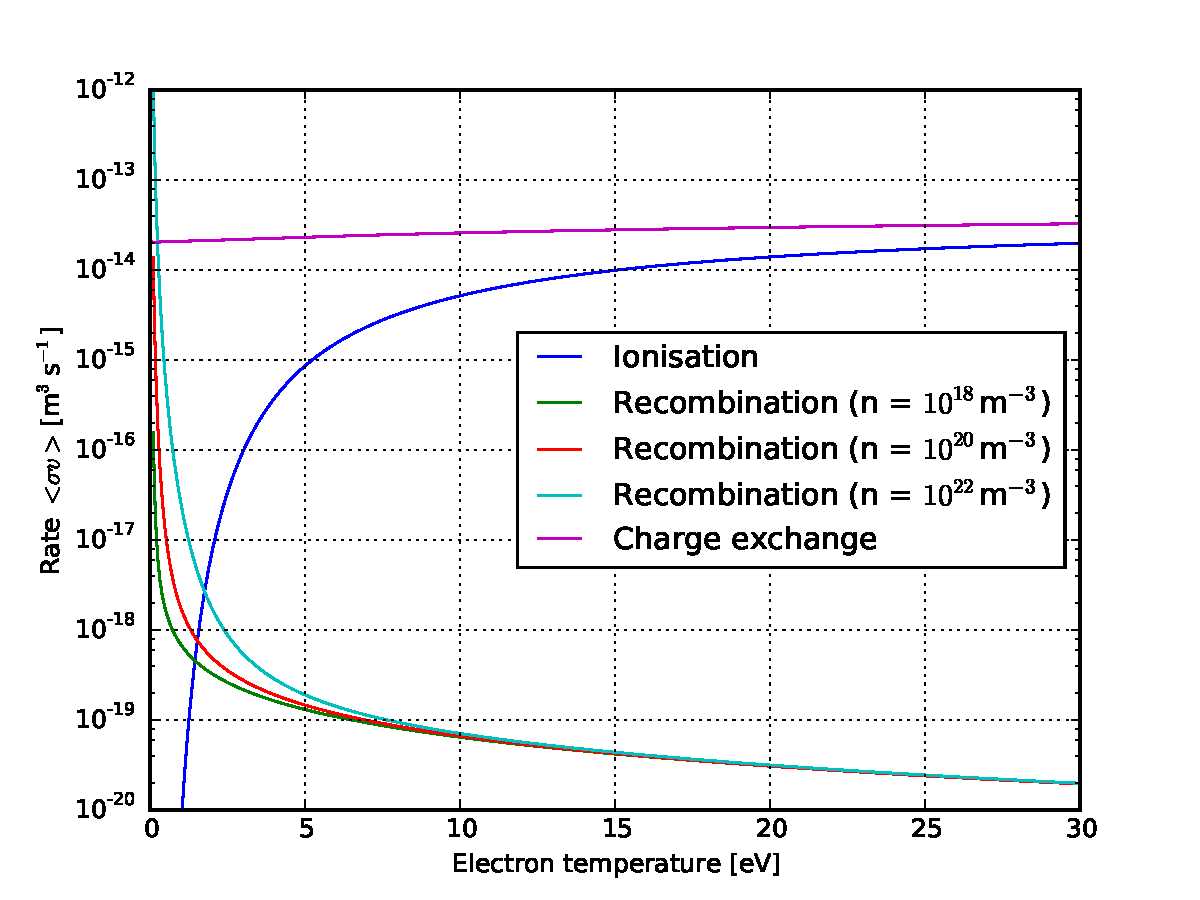
\includegraphics[width=0.7\columnwidth]{hydrogen.pdf}
\caption{Cross-sections [Thanks to E.Havlickova]}
\label{fig:sigma}
\end{figure}
Plots of these cross-sections are shown in figure~\ref{fig:sigma}. There are a few anomalies with this: charge exchange always has the highest cross-section of any process, and ionisation has a jump at $20$eV. The ionisation and
charge exchange rates do not depend on density, but recombination does so a typical range of values is shown.


\end{document}
